\section{The experimental setup}

\begin{figure}
    \centering
    \begin{subfigure}[b]{0.4\textwidth}
        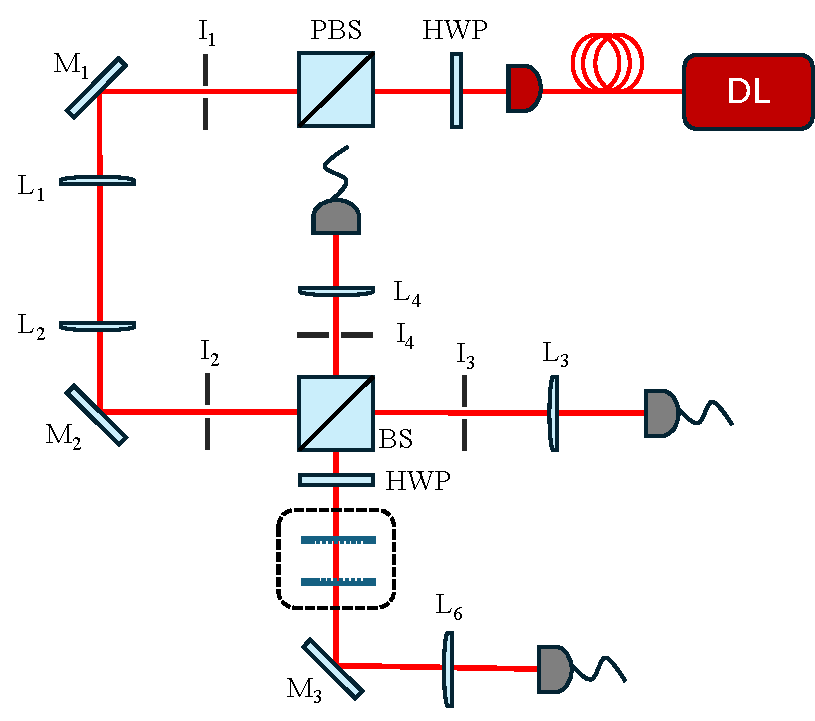
\includegraphics[width=\textwidth]{figures/setup_sketch.pdf}
        \caption{Schematics of the experimental setup for measuringthe transmission through a double fano cavity. The cavity setup shown in (b) is located in position marked by the dotted line.}
    \end{subfigure}
    \hfill
    \begin{subfigure}[b]{0.59\textwidth}
        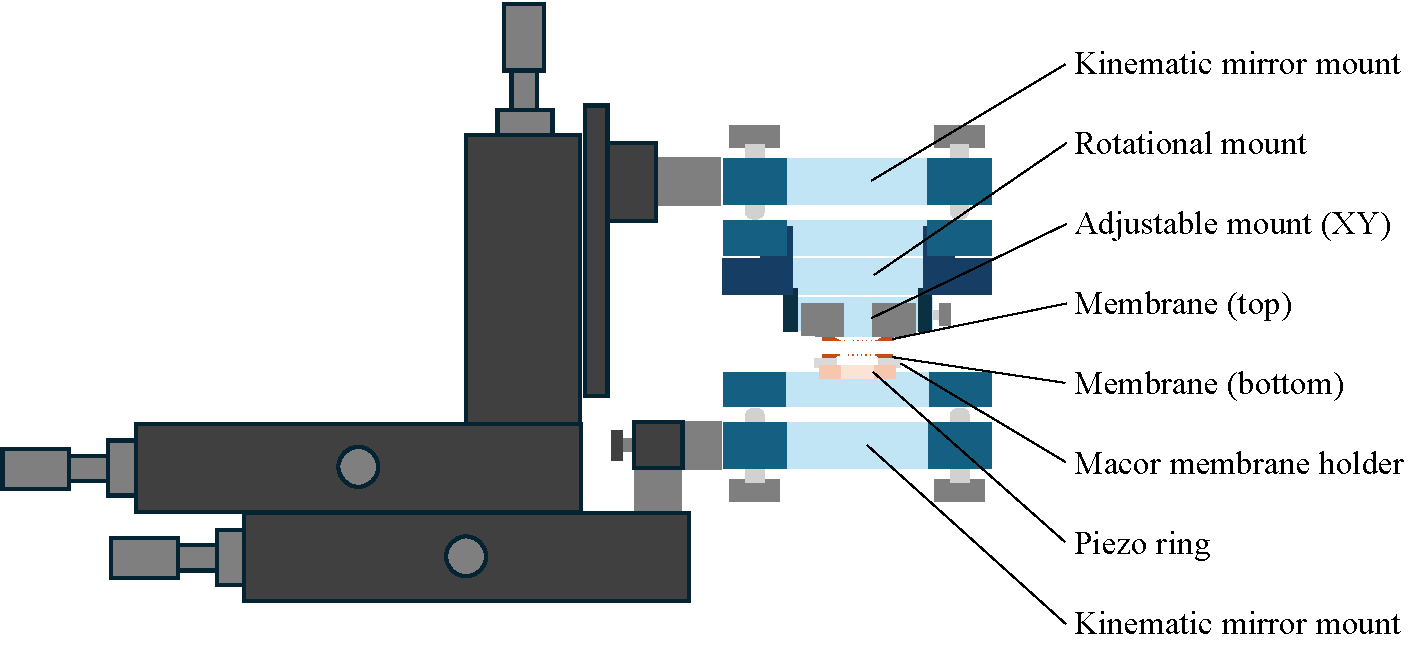
\includegraphics[width=\textwidth]{figures/setup_skecth_zoomed.pdf}
        \caption{Sketch of the part of the experimental setup containing the optical cavity.}
    \end{subfigure}
\end{figure}

\section{Characterization of sub-wavelength grating}

\subsection{Obtaining normalized transmission/reflection spectra}

\section{Cavity measurements}

\subsection{Parallelism study (deviation from normal incident)}

\subsection{Determining the cavity length from the FSR}

\subsection{Spacial drift of the piezo ring}

Figures: 
\begin{itemize}
    \item Linewidth as a function of "time" - to see the reduction of the linewidth as the piezo reaches an equilibrium where any time-dependent drift is reduced. 
\end{itemize}

\subsection{Single Fano cavity transmission} 

\subsection{Double Fano cavity transmission}

\subsubsection{Fabry-Perot cavity consisting of a grating and membrane (test of setup)}

\subsubsection{Off-resonance Fabry-Perot cavity (alignment technique)}

\subsubsection{Centering of the top grating (pinhole method)}

\subsubsection{Noise reduction (coupled mechanical/acoustic vibration and the plexi-glass box)} 